% Generated by figures/scripts/make_leaderboard_dev91.sh from figures/data/leaderboard_dev91.json; do not edit.
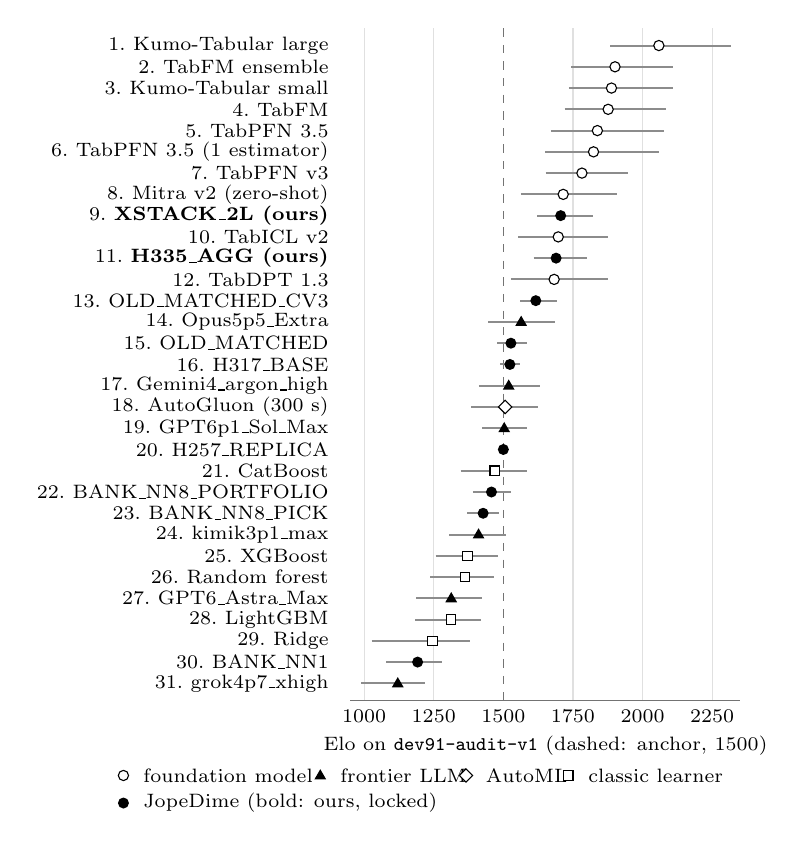
\begin{tikzpicture}[font=\scriptsize]
\draw[black!12,line width=0.4pt] (3.277,0.22) -- (3.277,-8.320);
\node[anchor=north] at (3.277,-8.320) {1000};
\draw[black!12,line width=0.4pt] (4.161,0.22) -- (4.161,-8.320);
\node[anchor=north] at (4.161,-8.320) {1250};
\draw[black!55,dashed,line width=0.4pt] (5.045,0.22) -- (5.045,-8.320);
\node[anchor=north] at (5.045,-8.320) {1500};
\draw[black!12,line width=0.4pt] (5.929,0.22) -- (5.929,-8.320);
\node[anchor=north] at (5.929,-8.320) {1750};
\draw[black!12,line width=0.4pt] (6.813,0.22) -- (6.813,-8.320);
\node[anchor=north] at (6.813,-8.320) {2000};
\draw[black!12,line width=0.4pt] (7.696,0.22) -- (7.696,-8.320);
\node[anchor=north] at (7.696,-8.320) {2250};
\draw[black!55,line width=0.4pt] (3.10,-8.320) -- (8.05,-8.320);
\node[anchor=north] at (5.58,-8.640) {Elo on \texttt{dev91-audit-v1} (dashed: anchor, 1500)};
\node[anchor=east] at (2.95,0.000) {1.\ Kumo-Tabular large};
\draw[black!45,line width=0.7pt] (6.401,0.000) -- (7.940,0.000);
\draw[black,fill=white,line width=0.4pt] (7.020,0.000) circle (0.065);
\node[anchor=east] at (2.95,-0.270) {2.\ TabFM ensemble};
\draw[black!45,line width=0.7pt] (5.909,-0.270) -- (7.204,-0.270);
\draw[black,fill=white,line width=0.4pt] (6.463,-0.270) circle (0.065);
\node[anchor=east] at (2.95,-0.540) {3.\ Kumo-Tabular small};
\draw[black!45,line width=0.7pt] (5.877,-0.540) -- (7.198,-0.540);
\draw[black,fill=white,line width=0.4pt] (6.418,-0.540) circle (0.065);
\node[anchor=east] at (2.95,-0.810) {4.\ TabFM};
\draw[black!45,line width=0.7pt] (5.822,-0.810) -- (7.106,-0.810);
\draw[black,fill=white,line width=0.4pt] (6.376,-0.810) circle (0.065);
\node[anchor=east] at (2.95,-1.080) {5.\ TabPFN 3.5};
\draw[black!45,line width=0.7pt] (5.647,-1.080) -- (7.089,-1.080);
\draw[black,fill=white,line width=0.4pt] (6.239,-1.080) circle (0.065);
\node[anchor=east] at (2.95,-1.350) {6.\ TabPFN 3.5 (1 estimator)};
\draw[black!45,line width=0.7pt] (5.576,-1.350) -- (7.019,-1.350);
\draw[black,fill=white,line width=0.4pt] (6.190,-1.350) circle (0.065);
\node[anchor=east] at (2.95,-1.620) {7.\ TabPFN v3};
\draw[black!45,line width=0.7pt] (5.581,-1.620) -- (6.633,-1.620);
\draw[black,fill=white,line width=0.4pt] (6.043,-1.620) circle (0.065);
\node[anchor=east] at (2.95,-1.890) {8.\ Mitra v2 (zero-shot)};
\draw[black!45,line width=0.7pt] (5.268,-1.890) -- (6.487,-1.890);
\draw[black,fill=white,line width=0.4pt] (5.805,-1.890) circle (0.065);
\node[anchor=east] at (2.95,-2.160) {9.\ \textbf{XSTACK\_2L (ours)}};
\draw[black!45,line width=0.7pt] (5.473,-2.160) -- (6.183,-2.160);
\fill[black] (5.773,-2.160) circle (0.07);
\node[anchor=east] at (2.95,-2.430) {10.\ TabICL v2};
\draw[black!45,line width=0.7pt] (5.234,-2.430) -- (6.373,-2.430);
\draw[black,fill=white,line width=0.4pt] (5.742,-2.430) circle (0.065);
\node[anchor=east] at (2.95,-2.700) {11.\ \textbf{H335\_AGG (ours)}};
\draw[black!45,line width=0.7pt] (5.429,-2.700) -- (6.105,-2.700);
\fill[black] (5.715,-2.700) circle (0.07);
\node[anchor=east] at (2.95,-2.970) {12.\ TabDPT 1.3};
\draw[black!45,line width=0.7pt] (5.140,-2.970) -- (6.372,-2.970);
\draw[black,fill=white,line width=0.4pt] (5.690,-2.970) circle (0.065);
\node[anchor=east] at (2.95,-3.240) {13.\ OLD\_MATCHED\_CV3};
\draw[black!45,line width=0.7pt] (5.258,-3.240) -- (5.723,-3.240);
\fill[black] (5.457,-3.240) circle (0.07);
\node[anchor=east] at (2.95,-3.510) {14.\ Opus5p5\_Extra};
\draw[black!45,line width=0.7pt] (4.850,-3.510) -- (5.705,-3.510);
\fill[black] (5.271,-3.510) ++(0,0.08) -- ++(-0.075,-0.13) -- ++(0.15,0) -- cycle;
\node[anchor=east] at (2.95,-3.780) {15.\ OLD\_MATCHED};
\draw[black!45,line width=0.7pt] (4.969,-3.780) -- (5.350,-3.780);
\fill[black] (5.141,-3.780) circle (0.07);
\node[anchor=east] at (2.95,-4.050) {16.\ H317\_BASE};
\draw[black!45,line width=0.7pt] (5.006,-4.050) -- (5.258,-4.050);
\fill[black] (5.128,-4.050) circle (0.07);
\node[anchor=east] at (2.95,-4.320) {17.\ Gemini4\_argon\_high};
\draw[black!45,line width=0.7pt] (4.734,-4.320) -- (5.510,-4.320);
\fill[black] (5.113,-4.320) ++(0,0.08) -- ++(-0.075,-0.13) -- ++(0.15,0) -- cycle;
\node[anchor=east] at (2.95,-4.590) {18.\ AutoGluon (300 s)};
\draw[black!45,line width=0.7pt] (4.639,-4.590) -- (5.480,-4.590);
\draw[black,fill=white,line width=0.4pt] (5.068,-4.590) ++(0,0.085) -- ++(0.085,-0.085) -- ++(-0.085,-0.085) -- ++(-0.085,0.085) -- cycle;
\node[anchor=east] at (2.95,-4.860) {19.\ GPT6p1\_Sol\_Max};
\draw[black!45,line width=0.7pt] (4.777,-4.860) -- (5.351,-4.860);
\fill[black] (5.056,-4.860) ++(0,0.08) -- ++(-0.075,-0.13) -- ++(0.15,0) -- cycle;
\node[anchor=east] at (2.95,-5.130) {20.\ H257\_REPLICA};
\draw[black!45,line width=0.7pt] (5.045,-5.130) -- (5.045,-5.130);
\fill[black] (5.045,-5.130) circle (0.07);
\node[anchor=east] at (2.95,-5.400) {21.\ CatBoost};
\draw[black!45,line width=0.7pt] (4.503,-5.400) -- (5.346,-5.400);
\draw[black,fill=white,line width=0.4pt] (4.935,-5.400) ++(-0.06,-0.06) rectangle ++(0.12,0.12);
\node[anchor=east] at (2.95,-5.670) {22.\ BANK\_NN8\_PORTFOLIO};
\draw[black!45,line width=0.7pt] (4.657,-5.670) -- (5.143,-5.670);
\fill[black] (4.894,-5.670) circle (0.07);
\node[anchor=east] at (2.95,-5.940) {23.\ BANK\_NN8\_PICK};
\draw[black!45,line width=0.7pt] (4.585,-5.940) -- (4.991,-5.940);
\fill[black] (4.788,-5.940) circle (0.07);
\node[anchor=east] at (2.95,-6.210) {24.\ kimik3p1\_max};
\draw[black!45,line width=0.7pt] (4.357,-6.210) -- (5.075,-6.210);
\fill[black] (4.730,-6.210) ++(0,0.08) -- ++(-0.075,-0.13) -- ++(0.15,0) -- cycle;
\node[anchor=east] at (2.95,-6.480) {25.\ XGBoost};
\draw[black!45,line width=0.7pt] (4.186,-6.480) -- (4.979,-6.480);
\draw[black,fill=white,line width=0.4pt] (4.591,-6.480) ++(-0.06,-0.06) rectangle ++(0.12,0.12);
\node[anchor=east] at (2.95,-6.750) {26.\ Random forest};
\draw[black!45,line width=0.7pt] (4.116,-6.750) -- (4.932,-6.750);
\draw[black,fill=white,line width=0.4pt] (4.555,-6.750) ++(-0.06,-0.06) rectangle ++(0.12,0.12);
\node[anchor=east] at (2.95,-7.020) {27.\ GPT6\_Astra\_Max};
\draw[black!45,line width=0.7pt] (3.941,-7.020) -- (4.779,-7.020);
\fill[black] (4.383,-7.020) ++(0,0.08) -- ++(-0.075,-0.13) -- ++(0.15,0) -- cycle;
\node[anchor=east] at (2.95,-7.290) {28.\ LightGBM};
\draw[black!45,line width=0.7pt] (3.924,-7.290) -- (4.762,-7.290);
\draw[black,fill=white,line width=0.4pt] (4.380,-7.290) ++(-0.06,-0.06) rectangle ++(0.12,0.12);
\node[anchor=east] at (2.95,-7.560) {29.\ Ridge};
\draw[black!45,line width=0.7pt] (3.372,-7.560) -- (4.627,-7.560);
\draw[black,fill=white,line width=0.4pt] (4.144,-7.560) ++(-0.06,-0.06) rectangle ++(0.12,0.12);
\node[anchor=east] at (2.95,-7.830) {30.\ BANK\_NN1};
\draw[black!45,line width=0.7pt] (3.560,-7.830) -- (4.263,-7.830);
\fill[black] (3.956,-7.830) circle (0.07);
\node[anchor=east] at (2.95,-8.100) {31.\ grok4p7\_xhigh};
\draw[black!45,line width=0.7pt] (3.241,-8.100) -- (4.055,-8.100);
\fill[black] (3.704,-8.100) ++(0,0.08) -- ++(-0.075,-0.13) -- ++(0.15,0) -- cycle;
\draw[black,fill=white,line width=0.4pt] (0.22,-9.270) circle (0.065);
\node[anchor=west] at (0.35,-9.270) {foundation model};
\fill[black] (2.72,-9.270) ++(0,0.08) -- ++(-0.075,-0.13) -- ++(0.15,0) -- cycle;
\node[anchor=west] at (2.85,-9.270) {frontier LLM};
\draw[black,fill=white,line width=0.4pt] (4.57,-9.270) ++(0,0.085) -- ++(0.085,-0.085) -- ++(-0.085,-0.085) -- ++(-0.085,0.085) -- cycle;
\node[anchor=west] at (4.70,-9.270) {AutoML};
\draw[black,fill=white,line width=0.4pt] (5.87,-9.270) ++(-0.06,-0.06) rectangle ++(0.12,0.12);
\node[anchor=west] at (6.00,-9.270) {classic learner};
\fill[black] (0.22,-9.620) circle (0.07);
\node[anchor=west] at (0.35,-9.620) {JopeDime (bold: ours, locked)};
\end{tikzpicture}
